\documentclass{amsart}

%\documentclass[10 pt]{amsart}

\usepackage[ocgcolorlinks,linktoc=all]{hyperref}
\hypersetup{citecolor=blue,linkcolor=red}
\usepackage[parfill]{parskip}
\usepackage{graphicx}

%\usepackage{amsthm}
\usepackage{cleveref}
\crefname{lemma}{Lemma}{Lemmata}
\crefname{equation}{equation}{equations}

\newtheorem{theorem}{Theorem}
\newtheorem{lemma}[theorem]{Lemma}
\newtheorem{proposition}[theorem]{Proposition}
\newtheorem{corollary}[theorem]{Corollary}

\newtheorem*{thmA}{Theorem}
\newtheorem*{thmB}{Theorem}
\newtheorem*{rem}{Remark}
\newtheorem*{thmmain}{Theorem}
\newtheorem*{propmain}{Proposition}

\theoremstyle{definition}
\newtheorem{definition}[theorem]{Definition}
\newtheorem{example}[theorem]{Example}
\newtheorem{xca}[theorem]{Exercise}

\theoremstyle{remark}
\newtheorem{remark}[theorem]{Remark}

\numberwithin{equation}{section}

%Symbols
\renewcommand{\~}{\tilde}
\renewcommand{\-}{\bar}
\newcommand{\bs}{\backslash}
\newcommand{\cn}{\colon}
\newcommand{\sub}{\subset}

\newcommand{\N}{\mathbb{N}}
\newcommand{\R}{\mathbb{R}}
\newcommand{\Z}{\mathbb{Z}}
\renewcommand{\S}{\mathbb{S}}
\renewcommand{\H}{\mathbb{H}}
\newcommand{\C}{\mathbb{C}}
\newcommand{\K}{\mathbb{K}}
\newcommand{\Di}{\mathbb{D}}
\newcommand{\B}{\mathbb{B}}
\newcommand{\8}{\infty}

%Greek letters
\renewcommand{\a}{\alpha}
\renewcommand{\b}{\beta}
\newcommand{\g}{\gamma}
\renewcommand{\d}{\delta}
\newcommand{\e}{\epsilon}
\renewcommand{\k}{\kappa}
\renewcommand{\l}{\lambda}
\renewcommand{\o}{\omega}
\renewcommand{\t}{\theta}
\newcommand{\s}{\sigma}
\newcommand{\p}{\varphi}
\newcommand{\z}{\zeta}
\newcommand{\vt}{\vartheta}
\renewcommand{\O}{\Omega}
\newcommand{\D}{\Delta}
\newcommand{\G}{\Gamma}
\newcommand{\T}{\Theta}
\renewcommand{\L}{\Lambda}

%Mathematical operators
\newcommand{\INT}{\int_{\O}}
\newcommand{\DINT}{\int_{\d\O}}
\newcommand{\Int}{\int_{-\infty}^{\infty}}
\newcommand{\del}{\partial}

\newcommand{\inpr}[2]{\left\langle #1,#2 \right\rangle}
\newcommand{\fr}[2]{\frac{#1}{#2}}
\newcommand{\x}{\times}

\DeclareMathOperator{\dive}{div}
\DeclareMathOperator{\id}{id}
\DeclareMathOperator{\pr}{pr}
\DeclareMathOperator{\Diff}{Diff}
\DeclareMathOperator{\supp}{supp}
\DeclareMathOperator{\graph}{graph}
\DeclareMathOperator{\osc}{osc}
\DeclareMathOperator{\const}{const}
\DeclareMathOperator{\dist}{dist}
\DeclareMathOperator{\loc}{loc}

%Environments
\newcommand{\Theo}[3]{\begin{#1}\label{#2} #3 \end{#1}}
\newcommand{\pf}[1]{\begin{proof} #1 \end{proof}}
\newcommand{\eq}[1]{\begin{equation}\begin{alignedat}{2} #1 \end{alignedat}\end{equation}}
\newcommand{\IntEq}[4]{#1&#2#3	 &\quad &\text{in}~#4,}
\newcommand{\BEq}[4]{#1&#2#3	 &\quad &\text{on}~#4}
\newcommand{\br}[1]{\left(#1\right)}



%Logical symbols
\newcommand{\Ra}{\Rightarrow}
\newcommand{\ra}{\rightarrow}
\newcommand{\hra}{\hookrightarrow}
\newcommand{\mt}{\mapsto}

% Aleksandrov Reflection Macros
\DeclareMathOperator{\reflectionvector}{V}
\DeclareMathOperator{\reflectionangle}{\delta}
\newcommand{\reflectionplane}[1][\reflectionvector]{\ensuremath{P_{#1}}}
\newcommand{\reflectionmap}[1][\reflectionvector]{\ensuremath{R_{#1}}}
\newcommand{\reflectionset}[2][\reflectionvector]{\ensuremath{{#2}_{#1}}}
\newcommand{\reflectionhalfspace}[1][\reflectionvector]{\ensuremath{\reflectionset[{#1}]{H}}}
\DeclareMathOperator{\vertvec}{e}
\DeclareMathOperator{\origin}{O}
\DeclareMathOperator{\radialprojection}{\pi}
\DeclareMathOperator{\height}{h}
\DeclareMathOperator{\equator}{E}
\newcommand{\ip}[2]{\ensuremath{\langle{#1},{#2}\rangle}}
\DeclareMathOperator{\intersect}{\cap}
\DeclareMathOperator{\union}{\cup}
\DeclareMathOperator{\nor}{\nu}
\DeclareMathOperator{\basepoint}{p_0}
\DeclareMathOperator{\radialdistance}{r}

%Fonts
\newcommand{\mc}{\mathcal}
\renewcommand{\it}{\textit}
\newcommand{\mrm}{\mathrm}

%Spacing
\newcommand{\hp}{\hphantom}


\parindent 0 pt

\protected\def\ignorethis#1\endignorethis{}
\let\endignorethis\relax
\def\TOCstop{\addtocontents{toc}{\ignorethis}}
\def\TOCstart{\addtocontents{toc}{\endignorethis}}

%\usepackage[left=1in,right=1in,top=1in,bottom=1in]{geometry}
\begin{document}

\title[Ancient solutions to curvature flows in the sphere]
 {On the classification of ancient solutions to curvature flows on the sphere}

\curraddr{}
\email{}
\date{\today}

\dedicatory{}
\subjclass[2010]{}
\keywords{}

\begin{abstract}
We consider the evolution of hypersurfaces on the unit sphere $\mathbb{S}^{n+1}$ by smooth functions of the Weingarten map. We introduce the notion of `quasi-ancient' solutions, which plays a similar role as ancient solutions for flows that do not admit non-trivial ancient solutions. The techniques presented here allow us to prove that any convex, quasi-ancient solution of a curvature flow which satisfies a uniform bound on the second fundamental form backwards in time must be a family of shrinking geodesic spheres. The main tools are geometric and the maximum principle, using a rigidity result in the sphere and an Aleksandrov reflection argument.
\end{abstract}

\maketitle

\section{Introduction}
\label{sec:intro}

We consider the evolution of a hypersurface $M^n$ by
\eq{\label{eq:CurvFlow}
\partial_tx=-F(\mathcal{W})\nu,~ x:M^n\times[0,T)\to \S^{n+1},
}
where \(\S^{n+1}\) is equipped with the constant curvature one, round metric, \(\mathcal{W}\) is the Weingarten map and \(F : \Gamma(T^\ast M \otimes TM) \to C^{\infty}(M)\), so that for any diagonalisable \(A, B \in \Gamma(T^\ast M \otimes TM)\), we have
\[
A < B \Rightarrow F(A) < F(B)
\]
where \(A < B\) means that \(B - A\) has positive eigenvalues. Here, \(A\) diagonalisable means that \(TM\) splits completely into a sum of one-dimensional, \(A\) invariant sub-spaces, or equivalently in any local coordinates, the matrix representing \(A\) may is diagonalisable.

This latter condition ensures the flow is strictly parabolic. In particular, it also ensures that if \(M_t = x_t(M)\) is strictly convex, then \(F(\mathcal{W}) > 0.\) Since \(\mathcal{W}\) is symmetric, it is diagonalisable and so \(F\) induces a symmetric function on the eigenvalues. Conversely, any such function induces an \(F\). Expressed in terms of \((\kappa_1,\cdots,\kappa_n)\), the eigenvalues of \(\mathcal{W}\) (principal curvatures), the parabolicity condition translates to 
\[
\frac{\partial F}{\partial \kappa_i} > 0.
\]

We consider \emph{quasi-ancient}, strictly convex solutions of \eqref{eq:CurvFlow}. Here quasi-ancient refers to solutions existing on the same time interval as the maximal flow of geodesic spheres. For many common flows, such as the Mean Curvature Flow \(F(\mathcal{W}) = \text{Trace}(\mathcal{W}) = H\), the maximal flow of geodesic spheres is the infinite time interval \((-\infty, 0)\). However for flows \(F = H^p\) with \(p \in (0,1)\), the maximal time interval is in fact finite. See \cref{sec:quasi_ancient}.

We prove the following theorem,
\begin{thm}
Let \(M_t\) be a \emph{quasi-ancient}, strictly convex solution of \eqref{eq:CurvFlow} with bounded mean curvature. Them \(M_t\) is a flow of shrinking geodesic spheres.
\end{thm}

In certain situations, such as concave speeds with speed comparable to \(H\), or one-homogeneous convex speeds, the theorem is actually quite easy to prove and we offer a short proof in this case in \cref{sec:convex_concave_homogeneous}. This should be compared, for instance with the result in \cite[Theorem]{HuiskenSinestrari:05/2014} where a short proof in the case of the Mean Curvature Flow in the sphere may be found. The main idea is to find the correct quantity to which the maximum principle may be applied. In the paper referred to, it is the pinching quantity, \((|A|^2 - n H^2)/H^2\) used so often for the Mean Curvature Flow. Here, we use \(\mathcal{W}/F\) for concave, mean curvature comparable speeds and the non-collapsing quantity \(k\) for one-homogeneous, convex speeds used in \cite{andrews2015Non-collapsing}.

The main thrust of the theorem, is that we have very strong rigidity in the sphere, and are able to prove the result in great generality - \emph{all we require is parabolicity of the flow}. At this level of generality, it is quite difficult to obtain suitable estimates, in particular Evans-Krylov higher regularity estimates are not known for arbitrary non-linear equations and hence less direct PDE methods are required. We obtain the theorem by first using the rigidity results of \cite{MakowskiScheuer:/2013} to argue that quasi-ancient solutions with bounded \(H\) must limit to an equator backwards in time. Then the Aleksandrov reflection technique developed in \cite{bryanlouie,2015arXiv150802821B} applies to show the symmetry is preserved under the flow, completing the classification. Let us remark that one may seek other methods of classification, using more PDE theoretic techniques, but they tend to suffer the draw back that they only apply (without modification) to speeds \(F\) that are non-singular and non-degenerate on the equator. The methods we describe here, apply even in the case of \emph{singular or degenerate speeds on the equator}. Very simple examples of such speeds are \(H^p\) which is singular for \(0 < p < 1\) and degenerate for \(p > 1\) whenever \(H = 0\), in particular along the equator. We find that the geometric methods are quite appealing and of interest in their own right, even in cases where PDE methods are applicable, these methods offering a powerful, complementary alternative to direct PDE techniques and supplanting them in cases where such methods are unknown.

One limitation of our method is that at this stage, we assume a bound on the mean curvature \(H\). Although there are certainly solutions emanating from convex polyhedra (and hence with unbounded \(H\)), it is not at all clear to us whether such solutions can be quasi-ancient. In \cref{sec:quasi} we give two examples (for non geometric flows) showing what could go wrong. The first converges to a lune, with unbounded \(H\) and the second converges to an equator, but is not a family of shrinking spheres. Since these examples are not geometric flows, they are not of the type considered here, but they do show that parabolic flows on the sphere may admit ancient solutions that are not a family of shrinking geodesics spheres.

It's also worth comparing the techniques and results here to the Euclidean case. The latter does not exhibit such strong rigidity and other ancient, convex solutions may occur. Indeed, for the Curve Shortening Flow in the plane, \cite{DaskalopoulosHamiltonSesum:2010} have classified all such solutions as either shrinking circles or the Angenent oval (also known as the paper clip solution) \cite{Angenent:1992}. In higher dimensions, \cite{HuiskenSinestrari:05/2014} and \cite{HaslhoferHershkovits:08/2013} have characterised when ancient, convex mean curvature flows are by shrinking spheres, and one would generally expect a greater variety of convex ancient solutions to exist. Convex, ancient solutions are of interest as they arise as rescalings of singularities \cite{HuiskenSinestrari:01/1999} of mean convex, mean curvature flow \cite{HuiskenSinestrari:09/1999, White:10/2002}. Singularity models for mean curvature flow in the sphere, have been studied in \cite{Nguyen:2015} where mean convex singularities with an ambient curvature dependent pinching condition are classified according to a blow-up yielding ancient solutions in Euclidean space, as opposed to the ancient, convex solutions in the sphere studied here.

This paper is laid out as follows: In \cref{prelim} we establish some notation and basic equations to be used in this paper. In \cref{quasi}, we introduce the notion of quasi-ancient solutions and establish some facts about such. Then in \cref{sec:concave_convex_homogeneous} we give a short classification result for concave and 1-homogeneous convex speeds. The following section, \cref{sec:rigidity} contains the rigidity results used to show backwards limits with bounded \(H\) are equators. Then finally in \cref{sec:reflection}, we used an Aleksandrov reflection technique to complete the classification.

\section*{Acknowledgment}

The authors would like to thank Knut Smoczyk and the Institut f\"{u}r Differentialgeometrie at Leibniz Universität for hosting a research visit where part of this work took place. The first author was a Riemann Fellow at the Riemann Center for Geometry and Physics, Leibniz Universit\"{a}t and was also supported by the EPSRC on a Programme Grant entitled ``Singularities of Geometric Partial Differential Equations'' reference number EP/K00865X/1. The work of the second author was supported by Austrian Science Fund (FWF) Project M1716-N25.

\section{Preliminaries}
\label{sec:prelim}

We will need some notation for derivatives of the speed \(F\). Let us write
\[
F^{i}_{j} = \frac{\partial F}{\partial h^{j}_{i}}
\]
for the first partial derivatives of \(F\). As a function of the metric and second fundamental form,
\[
F(g, h) = F(g^{ik} h_{kj}),
\]
we write
\[
F^{ij} = \frac{\partial F}{\partial h_{ij}}, \quad F^{ij,kl} = \fr{\partial^2F}{\partial h_{kl} \partial h_{ij}}.
\]
Let us also define the operator
\[
\Box = F^{ij} \nabla^2_{ij}.
\]
\begin{lemma} \label{lem: basi ev}
The following evolution equations hold:
\eq{
 \label{eq:delt_weingarten_box} 
\partial_t h_i^j &= \Box h_i^j + F^{kl} (h^2)_{kl} h_i^j - (F^{kl}h_{kl} - F) (h^2)_i^j + F^{kl,rs}\nabla_i h_{kl}\nabla^j h_{rs} \\
& \quad + K \{(F + F^{kl}h_{kl}) \delta_i^j - \p^{kl}g_{kl} h_i^j\},
}
\eq{\label{eq:delt_speed} \partial_t F = \Box F + FF^{ij}(h^2)_{ij} + K FF^{ij}g_{ij}.}
\end{lemma}

We will have occasion to work with graphs \(u\) over an equator, \(E \subset \mathbb{S}^{n+1}\).

A straightforward computation yields the following representation of the Weingarten map in terms of the function $u,$ namely
\eq{\label{graph h}h^i_j=\fr{\vt'}{v\vt}\d^i_j+\fr{\vt'}{v^3\vt^3}\nabla^iu\nabla_ju-\fr{\~g^{ik}}{v\vt^2}\nabla^2_{kj}u,}
where $\~g^{ij}$ is the inverse of $\~g_{ij}=\vt^{-2}g_{ij}$, $\vt(r)=\sin r$ and \(v^{-1} = \partial_r \cdot \nu\). Covariant derivatives as well as index raising is performed with respect to $\s_{ij}$, the round metric on the equator, \(E \simeq \S^n\). Compare for example \cite[(3.82)]{Scheuer:05/2015}.

A one-parameter family of graphs satisfying the flow \eqref{eq:CurvFlow}, thus is a solution of
\begin{equation}
\label{eq:GraphCurvFlow}
\fr{\del}{\del t}u=-F\br{\fr{\vt'}{v\vt}\d^{i}_{j}+\fr{\vt'}{v^{3}\vt^{3}}\nabla^{i}u\nabla_{j}u+\fr{\~g^{ik}}{v\vt^{2}}\nabla^{2}_{kj}u}v=\Phi(x,u,\nabla u,\nabla^{2}u).
\end{equation}

The paraboicity assumption is that \(dF > 0\), and writing,
\[
\Phi = \Phi(x, r, p, z)
\]
we find that linearising around \(u_0\) symbol is,
\[
\sigma(u_0) \cdot X = d\Phi_z \cdot X = dF \cdot \fr{1}{v(u_0) \vt^{2}(u_0)} \~g^{-1}(u_0) \cdot X
\]
for \(X \in TC^{\infty}(E, \mathbb{R}) \simeq C^{\infty}(E, \mathbb{R})\). This is uniformly elliptic wherever \(\~g^{-1}(u_0)\) is, and wherever, \(v(u_0), \vt(u_0)\) are bounded below. In particular, this is true if the hypersurface represented by the graph \(u_t\) is strictly convex with second fundamental form, uniformly \(h(u_t)\) bounded below.

In particular, we may apply the maximum principle \cite[Theorem 3.1.1]{Giga:2006} as follows.

\begin{thm}
\label{thm:comparison}
Let \(u_t, v_t\) be strictly convex solutions of \eqref{eq:CurvFlow} on a domain \(\Omega_t \subset E\) such that \(u_t \leq v_t\) on the parabolic boundary. Then \(u_t \leq v_t\) on all \(\Omega_t\).
\end{thm}

\begin{proof}
Do we need to show that a lower bound on \(\mathcal{W}\) is preserved along the flow? NO! Degenerate elliptic (not uniformly!) is all we need.
To apply the maximum principle \cite[Theorem 3.1.1]{Giga:2006}, we need to verify the following conditions:
- (F1) Continuity of \(\Phi\). Follows from the continuity of \(F\) and the smoothness of the solution,
- (F2) Degenerate Elliptic. Follows from the fact that \(\~g^{-1}\) is elliptic and \(F\) is monotone,
- (F3) Bounded.
- (F4) Monotone. By smoothness, on any finite time interval, \([-T_1, -T_2]\), everything is bounded hence we can choose a constant large enough so this condition is satisfied.
{\color{red} Giga assumes independence of $x,$ which is not given here.}
\end{proof}

\section{Ancient and quasi-ancient Solutions}
\label{sec:quasi_ancient}

We consider the spherical ambient space, $K=1,$ without further mention, and we are interested in solutions with maximal possible lifetime. To understand this maximal time, we define $T_S$ to be the lifespan of \it{the} convex spherical solution of \eqref{eq:CurvFlow}. By the convex spherical solution we mean a family of geodesic spheres shrinking under the flow \eqref{eq:CurvFlow} collapsing to a point at time $t=0$ and existing on the maximal interval \((-T_S, 0)\). For some speeds, \(T_S\) is finite.

\begin{lemma}
 Consider \eqref{eq:CurvFlow} with speed \(F = f^p\) with \(f\), convex, 1-homogeneous, and \(p \in (0,1)\). Then a flow of strictly convex geodesic spheres has a finite lifespan, i.e., let $S_r(p)$ be a geodesic sphere in $\S^{n+1}$. Then the flow exists only for a finite time interval \((-T_S,0)\) with \(0 < T_S < \infty\), collapsing to a point at \(t=0\) and converging to an equator at \(t=T_S\).
\end{lemma}

\begin{proof}
We may assume that $f(1,\cdots,1)=n.$
Since $F$ is constant on a geodesic sphere, the evolution equation (\ref{lem: basi ev}) for a flow of geodesic spheres yields
\eq{\fr{d}{dt}f\geq nf^{p}.}
Since the right hand side remains strictly positive under this ODE, we obtain finite lifespan forward in time.
Convexity and integration over some interval $(a,b)$ yield
\eq{0\leq f^{1-p}(a)\leq f^{1-p}(b)-n(1-p)(b-a).}
Allowing $a\ra-\8$ gives the finite existence backwards in time.
\end{proof}

\begin{lemma}
Let $x$ be a convex solution of \eqref{eq:CurvFlow}, defined on the open interval $(-T,0),$ where $0$ is the collapsing time, then $T\leq T_S.$
\end{lemma}

\begin{proof}
Suppose $T>T_S+\e$ for some $\e>0$. Since $M=M_{-T_S-\fr{\e}{2}}$ bounds a convex body $\hat{M}$, it is strictly contained in an open hemisphere due to the classical paper \cite{CarmoWarner:/1970}. Then there exists a geodesic sphere $S$ with $\hat{M}\sub\hat{S}.$ By the avoidance principle, the flow with initial hypersurface $M$ collapses before the spherical flow and thus contradicting $T>T_S$.
\end{proof}

Due to this lemma, the following definition is reasonable.

\begin{defn}
A convex solution of \eqref{eq:CurvFlow} defined on maximal interval $(-T,0)$ is called \it{quasi-ancient}, if $T=T_S$.
\end{defn}

The term ancient is reserved for the situation when \(T_S=\infty\), and by the definition, ancient solutions are also quasi-ancient.

For 1-homogeneous, convex speeds, Proposition \ref{cor:boundedH} to follow gives a bound on mean curvature for ancient solutions. For quasi-ancient solutions, the Harnack inequality does not, in general, give such a bound, since we cannot send \(t \to -\infty\) whenever \(T_S\) is finite. One can envisage backwards limits as convex polyhedra and hence with unbounded \(H\), but it is not clear that these solutions exist on the maximal time interval \((-T_S, 0)\), i.e. are quasi-ancient solutions. For the purposes of classification of quasi-ancient solutions, we make the additional assumption that \(H\) is bounded, and defer the question of whether solutions with unbounded \(H\) can exist to a later date.

\begin{prop}
\label{cor:boundedH}

Suppose $F$ is a \(1\)-homogeneous, convex function. Then any convex ancient solution of the contracting flow with speed $F$ satisfies
\[\partial_t F-b^{ij}\nabla_i F \nabla_j F \geq 0.\]
In particular, for all $t\le -1$ we have
$H(\cdot,t)\leq c.$
Here $c<\infty$ depends only on $M_{-1}.$
\end{prop}

\begin{proof}
For any $t>s$, the  Harnack estimate of \cite[Theorem 1]{bryan2015harnack} implies that
$$\partial_t F-b^{ij}\nabla_i F\nabla_j F+\frac{n}{2}\frac{F}{t-s}>0.$$
Allowing $s\to-\infty$ proves the first claim. For the second claim, observe that for any 1-homogeneous, convex $F$ we have \[F\ge \frac{F(1,\cdots,1)}{n}H,\]
see \cite[Chapter 2]{Gerhardt:/2006}. Therefore, ancient solutions satisfy
\[H(\cdot,t)\leq \frac{n}{F(1,\cdots,1)}F(\cdot,t)\leq \frac{n}{F(1,\cdots,1)}F(\cdot,0). \]
\end{proof}

Let us round out this section by looking at some examples of flows for which our techniques do not apply, and the ``undesirable'' behaviour ruled out by our assumptions occurs. First, we have a flow is parabolic, but not geometric, and for which \(H\) becomes unbounded. As mentioned earlier, we do not yet know whether such singular behaviour can occur for isotropic, geometric flows.

\begin{example}
We consider a family of convex curves $\gamma_t$ on $\mathbb{S}^2$ that their spherical radial functions evolve by
\[\rho:\mathbb{S}^1\times[0,T)\to \mathbb{R}\]

\begin{equation}\label{eq: angenent oval}
\partial_t\rho(\cdot,t)=-\kappa \frac{\sqrt{\sin^2\rho+\rho_{\theta}^2}}{\sin\rho}\frac{\sin^2\rho+\rho_{\theta}^2}{\tan^2\rho+(\tan\rho)_{\theta}^2}(\cdot,t).
\end{equation}

Here, $\kappa(\cdot,t)$ is the curvature of the curve $\gamma_t$ with the radial function $\rho(\cdot,t).$ 
In the polar coordinates, we can express the curvature as follows:
\[\kappa=\frac{-\rho_{\theta\theta}\sin\rho+2\rho_\theta^2\cos\rho+\cos\rho\sin^2\rho}{(\sin^2\rho+\rho_{\theta}^2)^{\frac{3}{2}}}.\]

We will show that the gnomonic projection of $\gamma_t$, denoted by $\bar{\gamma}_t$, evolves by the curve shortening flow in $\mathbb{R}^2.$ Write $\bar{\rho}(\cdot,t)$ for the radial function of $\bar{\gamma}_t$. We recall from \cite[page 8]{besau2014spherical} that
$\bar{\rho}=\tan\rho.$ Using this formula and the expression of $\kappa$ we can write the curvature of $\bar{\gamma}_t$,  $\bar{\kappa}(\cdot,t),$ as follows:
\[\kappa=\left(\frac{\bar{\rho}^2+\bar{\rho}_{\theta}^2}{(1+\bar{\rho}^2)(\sin^2\rho+\rho_{\theta}^2)}\right)^{\frac{3}{2}}\bar{\kappa}=\left(\frac{\bar{\rho}^2+1}{\bar{h}^2+1}\right)^{\frac{3}{2}}\bar{\kappa}.\]
Here $\bar{h}=\frac{\bar{\rho}}{\sqrt{\bar{\rho}^2+\bar{\rho}_{\theta}^2}}$ is the support function of $\bar{\gamma}.$
Therefore, 
\begin{align*}
\partial_t\bar{\rho}&=-\bar{\kappa}(1+\bar{\rho}^2)\left(\frac{\bar{\rho}^2+\bar{\rho}_{\theta}^2}{(1+\bar{\rho}^2)(\sin^2\rho+\rho_{\theta}^2)}\right)^{\frac{3}{2}}\frac{\sqrt{\sin^2\rho+\rho_{\theta}^2}}{\sin\rho}\frac{\sin^2\rho+\rho_{\theta}^2}{\tan^2\rho+(\tan\rho)_{\theta}^2}\\
&=-\bar{\kappa}(1+\bar{\rho}^2)^{\frac{3}{2}}\left(\frac{\bar{\rho}^2+\bar{\rho}_{\theta}^2}{(1+\bar{\rho}^2)(\sin^2\rho+\rho_{\theta}^2)}\right)^{\frac{3}{2}}\frac{\sqrt{\sin^2\rho+\rho_{\theta}^2}}{\bar{\rho}}\frac{\sin^2\rho+\rho_{\theta}^2}{\tan^2\rho+(\tan\rho)_{\theta}^2}\\
&=-\bar{\kappa}\frac{\sqrt{\bar{\rho}^2+\bar{\rho}_{\theta}^2}}{\bar{\rho}}.
\end{align*}

The curve shortening flow in $\mathbb{R}^2$ has non-trivial ancient solutions, the Angenent ovals. Thus, there exists a non-trivial convex ancient solution to the flow (\ref{eq: angenent oval}). This ancient solution converges backwards in time to a lune (the intersection of two hemispheres) with a pair of antipodal points at which \(\kappa\) is unbounded.
\end{example}

The second example, exhibits a flow for which the symmetry of the backwards limit is not preserved. That is, the backwards limit is an equator, yet the flow is not by geodesic spheres. Again, this flow is not geometric, and it's unclear whether such a solution can occur for geometric flows. Necessarily, our results for geometric flows imply such a solution, though converging to an equator in \(C^0\), would have unbounded \(H\) and hence not converge in \(C^2\).

\begin{example}
We consider a family of convex curves $\gamma_t$ on $\mathbb{S}^2$ that their spherical radial functions evolve by
\[\rho:\mathbb{S}^1\times[0,T)\to \mathbb{R}\]
\begin{equation}\label{eq: ellipse}
\partial_t\tan\rho(\cdot,t)=-\kappa^{\frac{1}{3}} \frac{\sqrt{\sin^2\rho+\rho_{\theta}^2}}{\sin\rho}(\cdot,t).
\end{equation}

The gnomonic projection of $\gamma_t$ evolves by the affine normal flow in $\mathbb{R}^2:$ 
\begin{align*}
\partial_t\bar{\rho}&=-\bar{\kappa}^{\frac{1}{3}}\frac{\sqrt{\bar{\rho}^2+\bar{\rho}_{\theta}^2}}{\bar{\rho}}.
\end{align*}
Origin-centered ellipses are ancient solutions to the affine normal flow in $\mathbb{R}^2$ \cite{Ivaki:2016}. Thus, there exists a non-trivial convex ancient solution to the flow (\ref{eq: ellipse}). This ancient solution converges backwards in time to an equator.
\end{example}

\section{Convex, Concave and Homogeneous Speeds}
\label{sec:convex_concave_homogeneous}

\begin{prop}
Let $F$ be concave and 
$\fr{H}{F}\leq c,$
or let $F$ be convex and \(1\)-homogeneous. Then any strictly convex ancient solution of the flow \eqref{eq:CurvFlow} with speed $F$ is a family of contracting geodesic spheres.
\end{prop}
\pf{
We first consider the case that $F$ is a concave function. The tensor
$w^j_i=\fr{h^j_i}{F}$
satisfies the evolution equation
\eq{\del_tw^j_i&=\Box w^j_i-2KF^{kl}g_{kl}w^j_i+2K\d^j_i\\
 &\hp{=}+F^{kl,rs}\nabla_ih_{kl}\nabla^jh_{rs}+2F^{kl}\nabla_kh^j_i\nabla_l\br{\fr{1}{F}}.}
Hence, due to the concavity of $F$ we have for fixed index $i:$
$$\del_t\br{w^i_i-\fr{1}{n}}\leq\Box\br{w^i_i-\fr{1}{n}}-2nK\br{w^i_i-\fr{1}{n}}+2F^{kl}\nabla_kh^i_i\nabla_l\br{\fr{1}{F}}.$$
At a spatial maximum of $w^i_i-\tfrac{1}{n}$ we have
$$0=\nabla_k \br{\fr{h^i_i}{F}}=\fr{\nabla_k h^i_i}{F}+h^i_i\nabla_k\br{\fr{1}{F}}.$$
and hence by the maximum principle we obtain the bound
$$w^i_i-\fr 1n\leq c_0e^{-2nKt},$$
where $c_0$ is the upper bound for the function on the left-hand side at $t=0.$
Starting the flow at an arbitrary $s<0$ we find
$$\fr{\k_n}{F}\leq \fr 1n+c_se^{-2nK(t-s)}.$$
If $K=1,$ letting $s\ra-\8,$ we obtain at every time $t<0$ that 
$$\k_n\leq \fr{F}{n}.$$
This is only possible for totally umbilical hypersurfaces, and the result follows since the only closed, totally umbilical hypersurfaces of the sphere are geodesic spheres.

Now suppose that $F$ is a convex function, 1-homogeneous function normalised so that $F(1,\cdots,1)=n$. The non-collapsing result of \cite[Theorem 1.1]{andrews2015Non-collapsing} states any ancient solution of the flow with a 1-homogeneous convex speed $F$ satisfies
\[\frac{\kappa_{\min}}{F}(x,t)\geq \frac{1}{n}+C(s)e^{-2n(t-s)},\]
where $|C(s)|\leq \frac{1}{n}+\frac{\kappa_{\min}}{F}(x,s)\leq \frac{1}{n}+\frac{\kappa_{min}}{\frac{F(1,\cdots,1)}{n}H}(x,s)\leq \frac{1}{n}+\frac{1}{F(1,\cdots,1)}.$
Therefore, allowing $s\to-\infty$ yields
\[\frac{\kappa_{\min}}{F}(x,t)\geq \frac{1}{n}.\]
This in turn implies that
\[\kappa_{\min}(x,t)\geq \frac{F}{n}(x,t)\geq \frac{F(1,\cdots,1)}{n}\frac{H}{n}(x,t)\geq \frac{F(1,\cdots,1)}{n} \kappa_{\min}(x,t).\]
On the other hand, since $F(1,\cdots,1)= n,$ we get
\[\kappa_{\min}(x,t)\geq \frac{F}{n}(x,t)\geq \frac{H}{n}(x,t)\geq \kappa_{\min}(x,t).\]
That is, $H\equiv n\kappa_{\min}$ and once again, the flow is by totally umbilical hypersurfaces, hence by geodesic spheres.
}

\section{Rigidity and Backwards Limit}

Now we turn to more general speeds, \(F\). The aim of this section is to prove that for a quasi-ancient solution of \eqref{eq:CurvFlow} the backwards limit of the flow hypersurfaces \it{with bounded mean curvature}, $M_t$ is an equator for $t\ra -T_S$. We will use the method of \cite{MakowskiScheuer:/2013} to achieve this.

\begin{lemma}\label{ISC}
Let $x$ be a quasi-ancient solution of \eqref{eq:CurvFlow}. Then there holds:
\begin{enumerate}
  \item For all $t_0<0$ there exists a uniform radius $R>0,$ such that the enclosed convex bodies $\hat{M}_t,$ $-T_S<t\leq t_0,$ of the flow hypersurfaces $M_t$ satisfy a uniform interior sphere condition with radius $R.$
  \item For every $y_0\in\mrm{int}~\hat{M}_{t_0}$ the hypersurfaces $M_t,$ $-T_S<t\leq t_0$ can be written as a graph in geodesic polar coordinates around $y_0$ and the corresponding graph functions satisfy uniform $C^2$-estimates.
\end{enumerate}
\end{lemma}
\pf{
Fix an interior point $y_0\in \mrm{int}~\hat{M}_{t_0}.$ Since for a contracting flow the enclosed convex bodies of the flow hypersurfaces are strictly decreasing, they are strictly increasing backwards in time. By \cite[Lemma~3.9]{MakowskiScheuer:/2013} there exists a closed hemisphere $\mc{H}(x_0),$ such that
\eq{\hat{M}_t\sub\mc{H}(x_0).}
In our situation all hypersurfaces $M_t,$ $-T_S<t\leq t_0,$ satisfy
\eq{B_{\e}(y_0)\sub \mrm{int}~\hat{M}_t}
and
\eq{B_{\e}(\hat{y}_0)\sub \hat{M}_t^c}
with a uniform $\e,$ where $\hat{y}_0$ denotes the antipodal point of $y_0.$
Now we prove the two claims.

(1)~Consider the stereographic projection with $\hat{y}_0$ corresponding to infinity. The image hypersurfaces are then strictly convex hypersurfaces in Euclidean space with uniformly bounded second fundamental form. Blaschke's rolling theorem, cf.~\cite{Blaschke:/1956}, gives the interior sphere condition.\\

(2)~
Write the $M_t$ as graphs in geodesic polar coordinates around $y_0,$
\eq{M_t=\{(r,x^i)\cn r=u(t,x^i)\},}
where $r$ describes the geodesic distance to $y_0.$ In these coordinates the spherical metric takes the form
\eq{d\-s^2=dr^2+\sin^{2}r\s_{ij}dx^idx^j,}
where $(\s_{ij})$ is the round metric of $\S^n.$

Hence on the set in which the $M_t$ range, the metrics $\-g_{ij}=\sin^2r\s_{ij}$ and $\s_{ij}$ are equivalent.
Due to \cite[Thm.~2.7.10]{Gerhardt:/2006} for all convex hypersurfaces $M_t$ the quantity
\eq{v^2=1+\-g^{ij}\nabla_iu\nabla_ju}
is uniformly bounded by a constant which only depends on $\e.$
Hence by the equivalence of norms the $M_t$ are uniformly $C^1$-bounded in the sense that the corresponding functions $u(t,\cdot)$ are uniformly $C^1(\S^n)$-bounded. Recalling equation, \eqref{eq:graph h}, due to the curvature estimates we obtain uniform $C^2(\S^n)$-estimates for \(u\).}
\begin{cor}\label{Backlimit}
Let $x$ be a quasi-ancient solution of \eqref{eq:CurvFlow}. Then there exists a unique backwards limiting hypersurface $M_{-T_S}$ and the flow hypersurfaces $M_t$ converge to $M_{-T_S}$ in $C^{1,\b},$ $0<\b<1,$ in the sense that for a common graph representation as in Lemma \ref{ISC} there holds
\eq{u(t,\cdot)\ra u(-T_S,\cdot)}
in the norm of $C^{1,\b}(\S^n).$
\end{cor}
\pf{
Due to the point-wise monotonicity of $u(t,\cdot)$ backwards in time, we obtain a point-wise limit. The $C^{1,\b}$-convergence follows from compactness.
}
\begin{thm}
\label{thm:backwardslimit}
The hypersurface $M_{-T_S}$, defined in Corollary \ref{Backlimit}, is an equator.
\end{thm}
\pf{
Since the convex bodies $\hat{M_t}$ are increasing backwards in time and due to the uniform convergence of $M_t$ to $M_{-T_S},$ the set
\eq{\hat{M}_{-T_S}:=\overline{\bigcup_{t<0}\hat{M}_t}}
is a compact body with
\eq{\del \hat{M}_{-T_S}=M_{-T_S}.}
Since $\mrm{int}(\hat{M}_{-T_S})$ is a strictly convex set, it is especially weakly convex in a hemisphere in the sense of \cite[Def.~3.2]{MakowskiScheuer:/2013}. Thus $\hat{M}_{-T_S}$ is a weakly convex body in a hemisphere. The proof of \cite[Lemma~6.1]{MakowskiScheuer:/2013} can literally be applied to show that $\hat{M}_{-T_S}$ satisfies a uniform interior sphere condition as well.
We can apply \cite[Thmeorem 1.1]{MakowskiScheuer:/2013} and obtain that $\hat{M}_{-T_S}$ is either strictly contained in an open hemisphere or is equal to a closed hemisphere. The first alternative is not possible since the solution is quasi-ancient. We conclude that $\del \hat{M}_{-T_S}=M_{-T_S}$ is an equator of $\S^{n+1}.$
}

\section{Aleksandrov Reflection and Classification}

In this section, use the result of Theorem \ref{thm:backwardslimit} to classify convex, embedded, (quasi-)ancient solutions of contracting curvature flows on \(\S^{n+1}\) as either equators or shrinking geodesic spheres. The proof uses Aleksandrov reflection as in \cite{bryanlouie,2015arXiv150802821B} to show that the symmetry of the backwards limit is preserved along the flow. Here we give a very general version with minimal assumptions on the flow: all we require is that the flow limits to an equator at $-T_S$ in \(C^0\), with uniform \(C^2\) bounds, and that the maximum principle holds forward in time.

\subsection{Notation}
We work on the $(n+1)$-dimensional unit sphere, embedded into $\R^{n+2}$ by the standard inclusion.
% $j,$
%\eq{j\cn \S^{n+1}\hra \R^{n+2}.}
Let
\eq{e=e_{n+2}=\br{0,\dots,0,1}\in \R^{n+2}.}
For a vector $V\in \S^{n+1}$ let
\eq{H_{V}^{\pm}=\{x\in\R^{n+2}\cn \pm\inpr{x}{V}>0\}.}
%and
%\eq{P_{V}=V^{\perp}.}
For a set $S\in \R^{n+2}$ let
\eq{S^{\pm}_{V}=S\cap H^{\pm}_{V}. }
We denote the equator in $\S^{n+1}$ around $e$ by
\eq{E=e^{\perp}\cap \S^{n+1}.}
Let $\d_{V}$ be the signed angle $V$ makes with the hyperplane $e^{\perp},$
\eq{\d_{V}=\arcsin\inpr{V}{-e}.}
The reflection map across the hypersurface $V^{\perp}$ is denoted by
\eq{R_{V}\cn\R^{n+2}&\ra \R^{n+2}\\
			x&\mt x-2\inpr{x}{V}V,}
which is an isometry of $\R^{n+2}.$
Finally, for $x\in \S^{n+1}\bs\{\pm e\},$
let $\g_{x}$ denote the unique geodesic in $\S^{n+1}$ from $e$ to $-e,$ which passes through $x$ and then define
\eq{\pr(x)=\begin{cases} y, & x\in \S^{n+1}\bs\{\pm e\}\\
				E, & x=e~\text{or}~x=-e,\end{cases}}
where $y\in E$ is the unique element on the image of $\g_{x}$ lying in $E.$

The reader may find it useful to refer to \Cref{fig:reflection} for the arguments in this section.
\begin{figure}[htb]
\centering
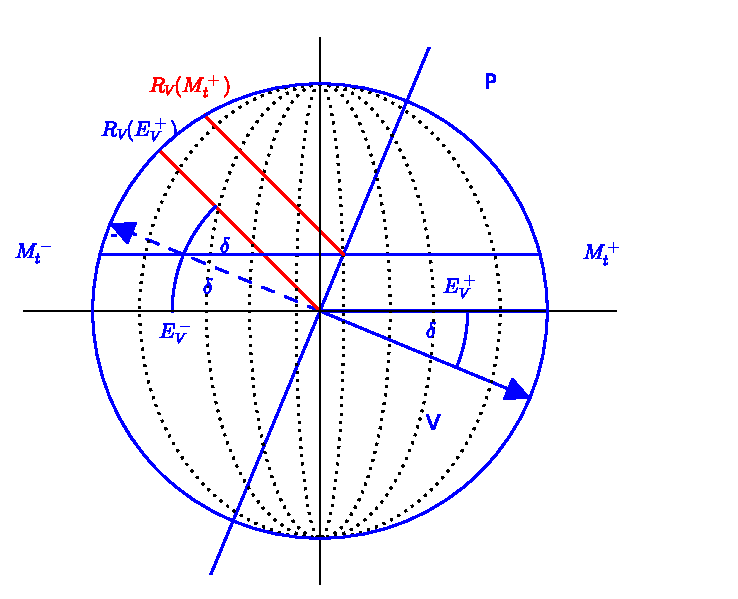
\includegraphics[width=.9\linewidth]{./reflection.pdf}
\caption{Reflection in the $(\vertvec, \reflectionvector)$-plane showing the reflected equator, \(M_T\), \(\reflectionmap(M_t)\) and some geodesics through the north pole (dotted lines).}
\label{fig:reflection}
\end{figure}

\subsection{Starshaped hypersurfaces and one-sided reflections}

\Theo{rem}{starshaped}{
Recall a nonempty set $S\in \S^{n+1}$ to be starshaped around $e,$ if $\pm e\notin S$ and if every geodesic from $e$ to $-e$ hits $S$ at most once, i.e.
\eq{\forall x\in E\cn \# \br{\mrm{Im}~\g_{x}\cap S}\leq 1.}
In this case we have a well-defined graph function of $S,$
\eq{f_{S}\cn \pr{S}&\ra \br{-\fr{\pi}{2},\fr{\pi}{2}}\\
			\s&\mt \arcsin\inpr{x_{\s}}{e}, }
where $x_{\s}$ is the unique preimage of $\s$ in $S$ under the projection $\pr.$ We obtain a parametrization of the set $S$ via the correspondance
\eq{x_{\s}=(\s,f_{S}(\s)).}
}

\Theo{defn}{ReflectsAbove}{
Let $S,T$ be starshaped sets around $e$ with corresponding graph functions $f_{S}$ and $f_{T}.$

(i)~We say \it{S lies above T}, written $S\geq T,$ if
\eq{\forall \s\in \pr{S}\cap\pr{T}\cn f_{S}(\s)\geq f_{T}(\s).}
(ii)~Let $V\in \R^{n+2}$ and suppose $R_{V}(S)$ and $R_{V}(T)$ are starshaped around $e.$ We say \it{S one-sided reflects above T}, if
\eq{R_{V}(S^{+}_{V})\geq T^{-}_{V}.}

}

\Theo{lemma}{Starshaped Reflection}{
Let $V\in\S^{n+1}$ and $0\leq\d\leq\d_{0}<\fr{\pi}{4}.$ Then

(i)~$R_{V}(E)$ is starshaped around $e.$

(ii)~There exists a constant $c=c(\d_{0})>0,$ such that for any closed and convex hypersurface $M\sub\S^{n+1}$ satisfying $e\notin M$ and
\eq{|f_{M}|\leq c,}
the reflection $R_{V}(M)$ is starshaped around $e.$
}

\pf{
(i)~Since $R_{V}(E)$ is also an equator, the only way not to be starshaped around $e$ would be
\eq{e\in R_{V}(E). }
But then, letting $e=R_{V}(x)$ with $x\in E,$
\eq{\sin \d_{V}=-\inpr{V}{e}=\inpr{x}{V}=\cos\d_{V},}
which is impossible in the given range of $\d_{V}.$

(ii)~The distance from $e$ to $R_{V}(E)$ only depends on $\d_{V}$ and thus for a sufficiently small graph function $f_{M}$ we also obtain $e\notin R_{V}(M).$ Since every convex hypersurface of the sphere is starshaped with respect to any interior (and exterior) point, the claim follows.
}

It is easily seen that the equator $E$ one-sided reflects above itself, if $0<\d_{V}<\fr{\pi}{4}.$ Now we show that this is also true for any convex hypersurface $M$ with controlled curvature, which is $C^{1}$-close to $E.$
The reason for these strong assumptions is the trouble that arises at the reflection plane $V^{\perp},$ at which the $M$ has the same height as its reflection.

\Theo{prop}{ReflectedM}{
For all $V\in\S^{n+1}$ with $0<\d_{1}\leq\d_{V}\leq \d_{0}<\fr{\pi}{4}$ and all $\Lambda>0$ there exists $\a=\a(\d_{0},\d_{1},\L)>0,$ such that all closed and convex hypersurfaces with $e\notin M,$
\eq{0\leq f_{M},\quad |f_{M}|_{C^{1}(M)}\leq\a\quad\text{and}\quad H\leq \L}
one-sided reflect above themselve. Here $H$ denotes the mean curvature of $M.$
}

\pf{By contradiction. Suppose there exists $V\in\S^{n+1}$ with $0<\d_{V}\leq \d_{0},$ $\Lambda>0$ and a sequence of hypersurfaces $M_{n}$ with
\eq{0\leq f_{M},\quad |f_{M_{n}}|_{C^{1}(M)}\leq \fr 1n,\quad H_{n}\leq \L,}
such that the $M_{n}$ do not one-sided reflect above themselve. This means that $R_{V}(M_{n}^{+})$ does not lie above $M_{n}^{-}$ (from now on we suppress the subscript $V$ for better readability). By \cref{ReflectsAbove} this means that there exist sequences
\eq{x_{n}\in M_{n}^{+},\quad y_{n}\in \mrm{Im}~\g_{R(x_{n})}\cap M_{n}^{-},}
such that
\eq{\inpr{R(x_{n})}{e}<\inpr{y_{n}}{e}.}
Thus
\eq{\inpr{x_{n}}{e}&=\inpr{R(R(x_{n}))}{e}\\
				&=\inpr{R(x_{n})}{e}-2\inpr{R(x_{n})}{V}\inpr{V}{e}\\
				&=\inpr{R(x_{n})}{e}-2\sin \d\inpr{x_{n}}{V}.}
Thus
\eq{0=\limsup_{n\ra\8}\inpr{x_{n}}{e}\leq -2\sin\d\limsup_{n\ra\8}\inpr{x_{n}}{V}\leq 0.}
Thus without loss of generality
\eq{\inpr{x_{n}}{V}\ra0,\quad x_{n}\ra x\in V^{\perp}\cap E.}
Hence we also obtain
\eq{R(x_{n})\ra x\quad\text{and}\quad y_{n}\ra x.}
Denote by $C_{n}=C_{n}(\t)$ the unique great circle in $E,$ parametrized by arc length and containing $\pr(x_{n})$ and $\pr(y_{n}),$ which amounts to smooth curves $\l_{n}$ in $M_{n}\hra \R^{n+2}$ and $\mu_{n}$ in $R_{V}(M_{n}),$ just by restricting the graph functions of $M_{n}$ and $R_{V}(M_{n})$ to $C_{n}.$
 Since $x_{n}\in H_{V}^{+}$ and $y_{n}\in H_{V}^{-},$ after a possible translation $\t\mt\t+\t_{0}$ we find a time $\t_{1}^{n}>0,$ such that
\eq{\l_{n}(0)\in V^{\perp},\quad \l_{n}(\t^{n}_{1})=y_{n}\quad\text{and}\quad \mu_{n}(\t^{n}_{1})=R(x_{n}).}
Define the function $\xi_{n}\cn (-\pi,\pi)\ra\R$ by
\eq{\xi_{n}(\t)=\inpr{\mu_{n}(\t)}{e}-\inpr{\l_{n}(\t)}{e}.}
Noting that $\xi_{n}(0)=0,$ we obtain the Taylor expansion
\eq{\xi_{n}(\t)=\xi_{n}'(0)\t+\xi_{n}''(\t_{n})\t^{2},\quad \t_{n}\in[0,\t^{n}_{1}].}
There holds
\eq{\xi_{n}'(0)=\inpr{\mu'_{n}(0)}{e}-\inpr{\l'_{n}(0)}{e}\geq c_{\d}>0,}
since the first term converges to the corresponding slope of $R(C),$ i.e.
\eq{\fr{d}{d\t}_{|\t=0}\inpr{R(C(-\t))}{e}=\fr{d}{d\t}_{|\t=0}2\sin \d\inpr{C(-\t)}{V}\equiv 2c_{\d}>0,}
and the second term converges to $0.$
The term $\xi''_{n}(\t_{n})$ is uniformly bounded by the assumption on the mean curvature. Hence the length of the interval containing $0,$ where $\xi_{n}>0,$ is uniformly bounded from below by a constant depending on $\d.$ Choosing $n$ large enough, $\t_{1}^{n}$ becomes as small as desired, a contradiction.
}

\subsection{Reflecting quasi-ancient curvature flows}

The final aim of this section is to show that for solution of a curvature flow equation defined on an interval $(-T_{S},0),$ which converges backwards to $E$ in $C^{1}$ and has bounded curvature, the flow hypersurfaces are invariant under reflection about every hyperplane $V^{\perp}$ with $V\in E.$ Hence we somehow need to let $\d$ go to zero in the preceding proposition. Unfortunately, until now we only obtain that for given $\d>0,$ all flow hypersurface in an interval $(-T_{S},T_{\d})$ one-sided reflect above themselves. Hence we can not deduce that any flow hypersurface has this property for $\d=0.$ We have to get rid of the dependence of $\d$ in the interval $(-T_{S},T_{\d}).$ In the following lemma we use the parabolic maximum principle to achieve this.

\Theo{lemma}{MPReflection}{
Let the closed and convex hypersurfaces $M_{t},$ $-T_{S}<t<0,$ satisfy the parabolic curvature flow equation
\eq{\dot{x}=-F(\cW)\nu}
in $\S^{n+1}$ and suppose
\eq{M_{t}\ra E,\quad t\ra -T_{S},}
in the sense that $e$ lies in the enclosed convex bodies of the $M_{t}$ for sufficiently small $t$ and the graph functions satisfy
\eq{|f_{M_{t}}|_{C^{1}(E)}\ra 0,\quad t\ra -T_{S}.}
 Furthermore suppose
 \eq{\limsup_{t\ra -T_{S}}H_{M_{t}}\leq\L<\8.}
 Then there exists $T>-T_{S},$ such that for all $V\in \S^{n+1}$ satisfying
 \eq{0<\d_{V}\leq \fr{\pi}{8},}
 $M_{t}$ one-sided reflects above itself for all $t\in (-T_{S},T).$
 }

\pf{
By \cref{Starshaped Reflection} and the $C^{1}$-convergence of $M_{t}$ we obtain $T>-T_{S},$ such that $M_{t}$ and $R_{V}(M_{t})$ are starshaped around $e$ for all $t\in (-T_{S},T).$ We show that this $T$ already has the desired property. By \cref{ReflectedM} we know that for given $V\in \S^{n+1}$ with (suppressing the subscript $V$ again)
\eq{0<\d\leq \fr{\pi}{8}}
 there exists $\~T_{\d}>-T_{S},$ such that $M_{t}$ one-sided reflects above itself for all $t\in (-T_{S},\~T_{\d}).$ Pick a $-T_{S}<T_{\d}<\~T_{\d}$ and define the domain
\eq{\O=\bigcup_{t\in(T_{\d},T)}\{t\}\times \pr(M_{t}^{-})\sub (-T_{S},T)\times E.}
Recall from \eqref{graph h} that the time dependent graph functions of the $M_{t}$ satisfy
\eq{\label{FullyNonlinear}\fr{\del}{\del t}f=F\br{\fr{\vt'}{v\vt}\d^{i}_{j}+\fr{\vt'}{v^{3}\vt^{3}}\nabla^{i}f\nabla_{j}f+\fr{\~g^{ik}}{v\vt^{2}}\nabla^{2}_{kj}f}=\Phi(x,f,\nabla f,\nabla^{2}f),}
where $\vt=\vt\br{\fr{\pi}{2}-f}=\sin\br{\fr{\pi}{2}-f}$ and $\~g^{ik}$ is elliptic.
Since the Weingarten operator is invariant under ambient diffeomorphisms, the reflected hypersurfaces $R_{V}(M_{t})$ satisfy the same curvature flow equation with corresponding graph function $\p$ also satisfying \eqref{FullyNonlinear}.

The comparison principle, \cref{thm:comparison} applied on the domain \(\union\limits_{t \in (-T_S + \epsilon_{\reflectionangle}, -T)} \radialprojection(\reflectionset(M_t)^-) \subseteq \equator\) yields that \(g_t \geq f_t\) holds forwards in time on all of \((-T_S + \epsilon_{\reflectionangle}, -T)\) hence on \((-T_S, -T)\).
}

\begin{thm}
\label{thm:classification}
Let \(M_t\) be a convex, embedded (quasi-)ancient solution of any (uniform whenever on uniformly convex hypersurfaces) parabolic equation on \(\S^{n+1}\) such that \(M_t \to \equator\) in \(C^1\) as \(t \to -T_S\) with uniform \(C^2\) bounds. Then \(M_t\) is a family of shrinking geodesic spheres emanating from the equator \(\equator\) at \(t=-T_S\).
\end{thm}

\begin{proof}
From \cref{MPReflection} we have \(\reflectionmap(\reflectionset{(M_t)}^+) \geq \reflectionset{(M_t)}^-\) everywhere for all \(t \in (-T_S, -T)\) and any \(\reflectionangle \in (0,\reflectionangle_0)\). By continuity therefore, sending \(\reflectionangle \to 0\) we have \(\reflectionmap(\reflectionset{(M_t)}^+) \geq \reflectionset{(M_t)}^-\) for all \(t \in (-T_S, -T)\)  and any \(\reflectionvector\) satisfying \(\ip{\reflectionvector}{\vertvec} = 0\).

Now, we need some simple properties of $\reflectionmap[\reflectionvector_0]$ following from the fact that $\ip{\reflectionvector}{\vertvec} = 0$:
\begin{itemize}
\item $\reflectionmap^2 = \id$,
\item $S \geq T \Rightarrow \reflectionmap(S) \geq  \reflectionmap(T)$,
\item $\reflectionmap = \reflectionmap[-\reflectionvector]$, and
\item $\reflectionset{S}^{\pm} = \reflectionset[-\reflectionvector]{S}^{\mp}$.
\end{itemize}
Thus we obtain,
\begin{align*}
\reflectionset{(M_t)}^+ &= \reflectionmap(\reflectionmap(\reflectionset{(M_t)}^+)) \geq \reflectionmap(\reflectionset{(M_t)}^-) \\
&= \reflectionmap[-\reflectionvector](\reflectionset[-\reflectionvector]{(M_t)^+}) \geq \reflectionset[-\reflectionvector]{(M_t)}^-\\
&= \reflectionset{(M_t)}^+.
\end{align*}
We must have equality all the way through and hence the middle line implies
\[
\reflectionmap[-\reflectionvector](\reflectionset[-\reflectionvector]{(M_t)^+}) = \reflectionset[-\reflectionvector]{(M_t)}^-
\]
for any $\reflectionvector$.

Thus \(M_t\) is invariant under \(\reflectionmap\) for any \(\reflectionvector\) satisfying \(\ip{\reflectionvector}{\vertvec} = 0\) and hence is a geodesic sphere for every \(t \in (-T_S, T)\) and by uniqueness of solutions, is a geodesic sphere for every \(t \in (-T_S, 0)\).
\end{proof}

\bibliographystyle{amsplain}
\bibliography{Bibliography.bib}


\end{document}
